\begin{figure*}[t]
	\centering
	\subfigure[Convergence Rate, MNIST.]
	{
		\label{fig:mnist_speed}
		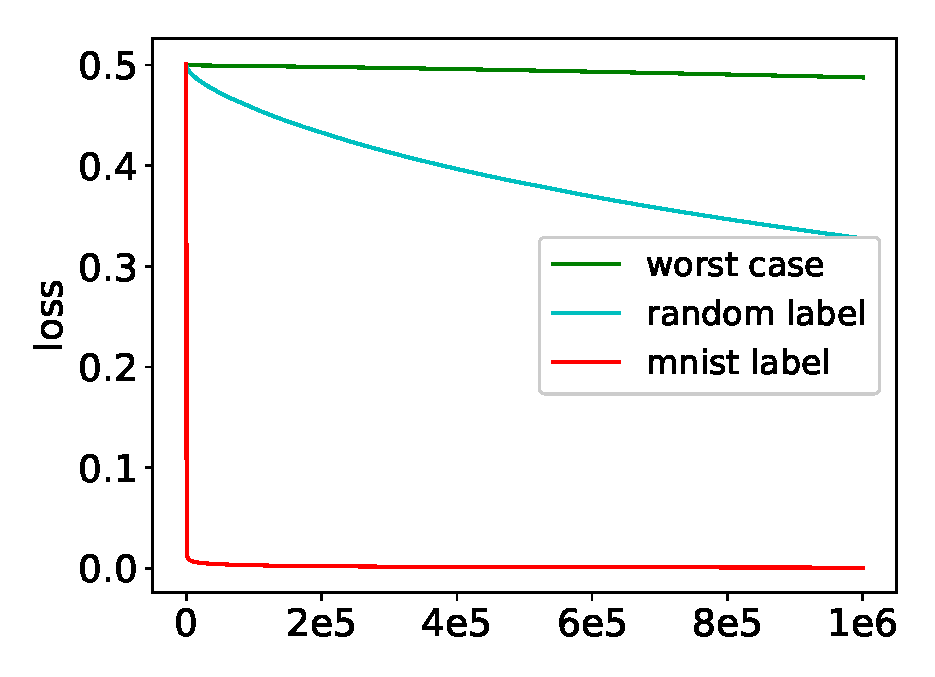
\includegraphics[width=0.4\textwidth]{figs/mnist_optimization.eps}}   
	\subfigure[Eigenvalues \& Projections, MNIST.]
	{
		\label{fig:mnist_spectrum}
		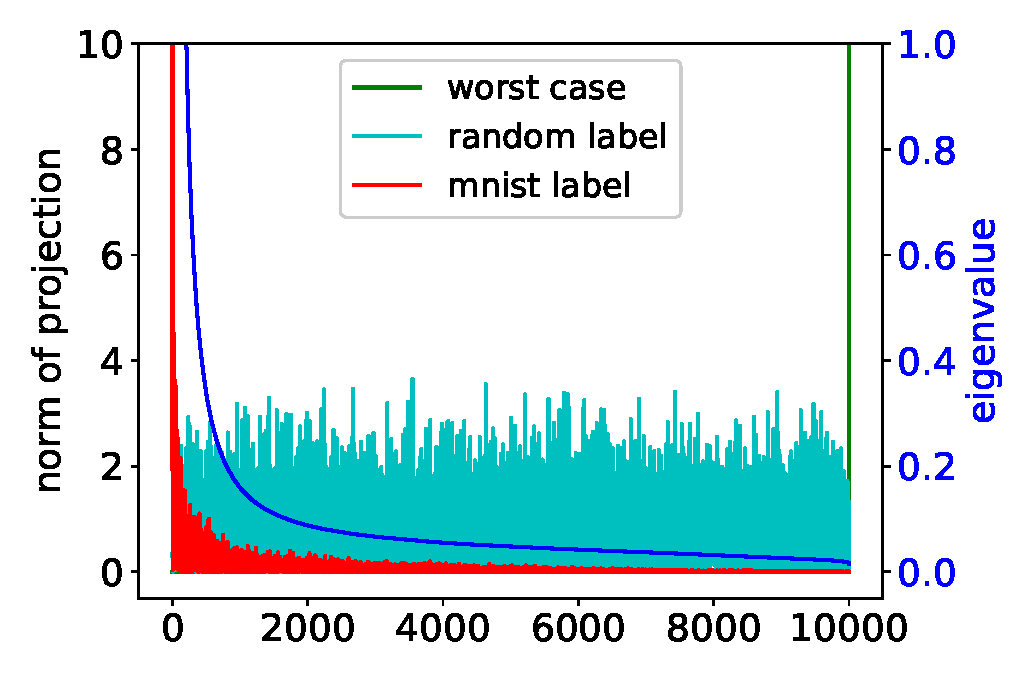
\includegraphics[width=0.44\textwidth]{figs/mnist_spectrum_proj.eps}}   \\
	\subfigure[Convergence Rate, CIFAR.]
	{
		\label{fig:cifar_speed}
		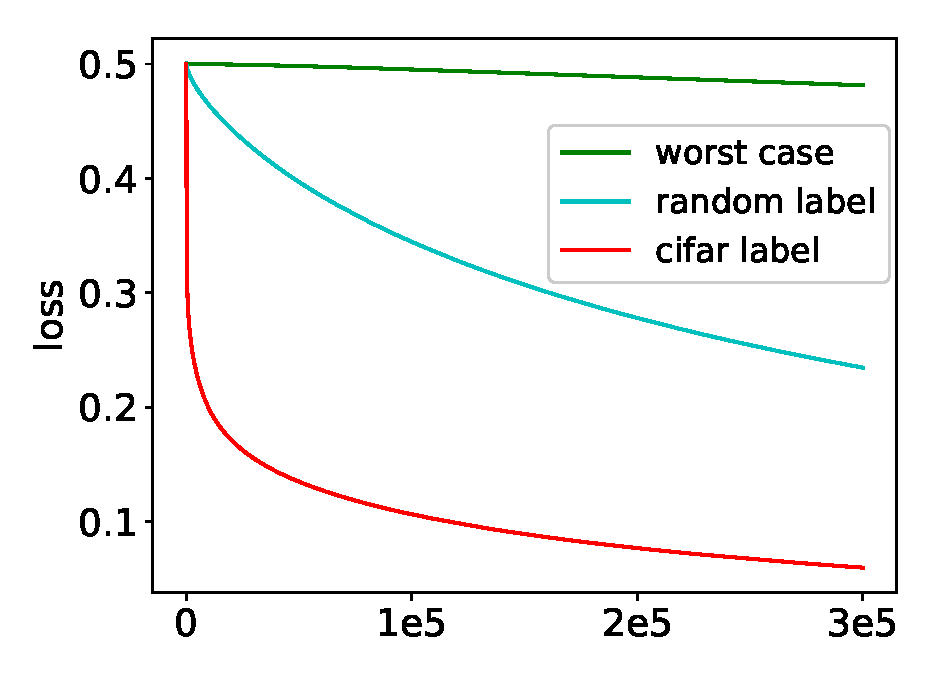
\includegraphics[width=0.4\textwidth]{figs/cifar_optimization.eps}}   
	\subfigure[Eigenvalues \& Projections, CIFAR.]
	{
		\label{fig:cifar_spectrum}
		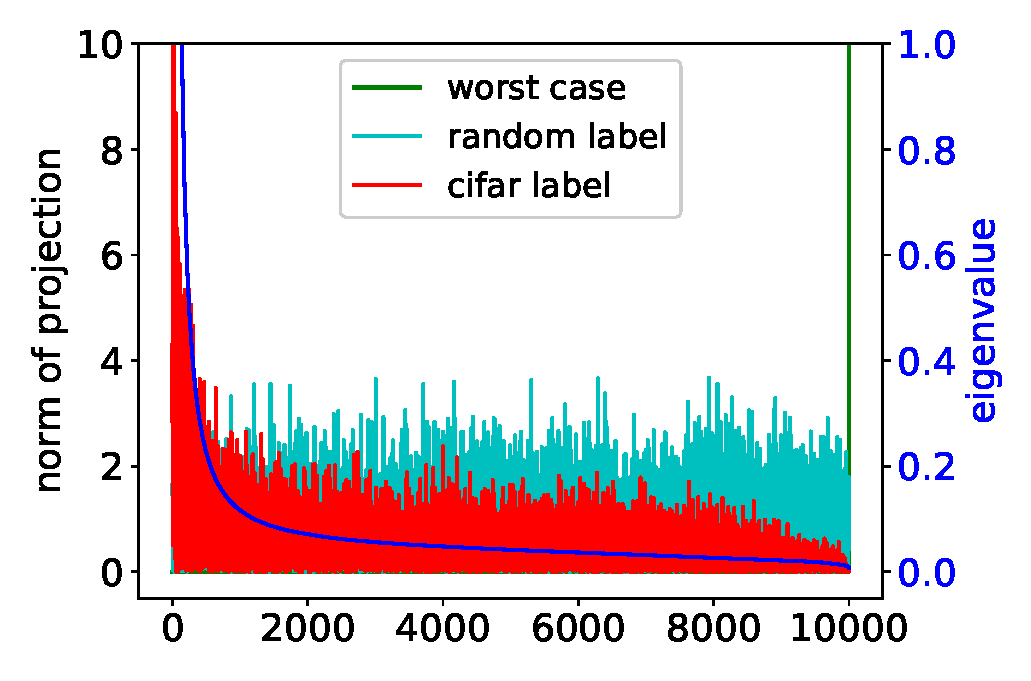
\includegraphics[width=0.44\textwidth]{figs/cifar_spectrum_proj.eps}}   
	\caption{In Figures~\ref{fig:mnist_speed} and \ref{fig:cifar_speed}, we compare  convergence rates of gradient descent between using true labels, random labels and the worst case labels (normalized eigenvector of $\vect{H}^\infty$ corresponding to $\lambda_{\min}(\mat{H}^{\infty})$.
		In Figures \ref{fig:mnist_spectrum} and \ref{fig:cifar_spectrum}, we plot the eigenvalues of $\mat H^\infty$ as well as projections of true, random, and worst case labels on different eigenvectors of $\vect{H}^{\infty}$. 
		The experiments use gradient descent on data from two classes of MNIST or CIFAR.
		%				, and the label of each data is set to $1$ or $-1$ according to each sample's category.
		The plots clearly demonstrate that true labels have much better alignment with top eigenvectors, thus enjoying faster convergence.
	}
	\label{fig:rate_mnist}
\end{figure*}


Although Theorem~\ref{thm:ssdu-converge} already predicts linear convergence of GD to $0$ loss, it only provides an upper bound on the loss and does not distinguish different types of labels. In particular, it cannot answer Question~\ref{ques:conv}.
In this section we give a fine-grained analysis of the convergence rate.

Recall the loss function $\Phi(\mat W) = \frac12 \norm{\vect y - \vect u}_2^2$.
%\begin{align*}
%L(\mat{W}) = \frac{1}{2}\sum_{i=1}^{n}\left(y_i-f(\vect{x}_i,\mat{W},\vect{a})\right)^2 = \frac{1}{2}\norm{\vect{y}-\vect{u}}_2^2.
%\end{align*}
Thus, %to study the convergence rate of gradient descent, we need to study how fast the sequence 
it is equivalent to study how fast the sequence $\left\{\vect{u}(k) \right\}_{k=0}^\infty$ converges to $\vect y$.
%$\left\{\norm{\vect{y}-\vect{u}(k)}_2^2\right\}_{k=0}^\infty$ converges to $0$.
Key to our analysis is the observation that when the size of initialization $\kappa$ is small and the network width $m$ is large, the sequence $\left\{\vect{u}(k) \right\}_{k=0}^\infty$ stays close to another sequence $\left\{\tilde{\vect{u}}(k)\right\}_{k=0}^\infty$ which has a \emph{linear} update rule:
\begin{equation}
\begin{aligned}
\tilde{\vect{u}}(0) &= \vect{0}, \\
\tilde{\vect{u}}(k+1) &= \tilde{\vect{u}}(k) - \eta \mat{H}^\infty\left(\tilde{\vect{u}}(k)-\vect{y}\right), \label{eqn:u_hat_dynamics}
\end{aligned}
\end{equation}
where $\mat H^\infty$ is the Gram matrix defined in~\eqref{eqn:H_infy_defn}.

Write the eigen-decomposition $\mat H^\infty = \sum_{i=1}^n \lambda_i \vect v_i \vect v_i^\top$, where $\vect v_1, \ldots, \vect v_n \in \R^n$ are orthonormal eigenvectors of $\mat H^\infty$ and $\lambda_1, \ldots, \lambda_n$ are corresponding eigenvalues.
Our main theorem in this section is the following:
%\begin{thm}\label{thm:convergence_rate}
%With at least $1-\delta$ probability over initialization, we have
%	\begin{align*}
%	\norm{\vect{y}-\vect{u}(k)}_2^2 
%	= &\norm{\vect{y}-\tilde{\vect{u}}(k)}_2^2 + \uerror(k)\\
%	= &\sum_{i=1}^{n}(1-\eta\lambda_i)^k \left(\vect{v}_i^\top \left(\vect{u}(0)-\vect{y}\right)\right)^2 + \uerror(k)
%	\end{align*}
%	where $\lambda_1 \ge \lambda_2 \ge \cdots \lambda_n \ge 0$ are eigenvalues of $\mat{H}^\infty$ and $\vect{v}_1,\vect{v}_2,\ldots,\vect{v}_n$ are corresponding eigenvectors and \begin{align*}
%		\abs{\uerror(k)} = O\left(k\left(1-\frac{\eta \lambda_0}{4}\right)^{k-1}\cdot\frac{\eta n^{5/2}\norm{\vect{y}-\vect{u}(0)}}{\sqrt{m}\delta\lambda_0}\right).
%	\end{align*}
%\end{thm}
\begin{thm}\label{thm:convergence_rate}
%	If $\initvar = \poly(\frac{1}{n},\delta,\lambda_0)$, then 
Suppose $\lambda_0 = \lambda_{\min}(\mat H^\infty) >0$,
$\kappa = O\left( \frac{\epsilon \delta}{\sqrt n} \right)$,
 $m = \Omega\left( \frac{n^7}{\lambda_0^4 \kappa^2 \delta^4 \epsilon^2} \right)$ and $\eta = O\left( \frac{\lambda_0}{n^2} \right)$. 
%Under the same assumptions as in Theorem~\ref{thm:ssdu-converge}, 
Then with probability at least $1-\delta$ over the random initialization, for all $k=0, 1, 2, \ldots$ we have: 
\begin{equation} \label{eqn:u(k)-y_size}
\norm{\vect{y}-\vect{u}(k)}_2
= \sqrt{\sum_{i=1}^{n}(1-\eta\lambda_i)^{2k} \left(\vect{v}_i^\top \vect{y}\right)^2} \pm \epsilon.
\end{equation}
%	\begin{equation} \label{eqn:u(k)-y_size}
%	\norm{\vect{y}-\vect{u}(k)}_2
%	= \sqrt{\sum_{i=1}^{n}(1-\eta\lambda_i)^{2k} \left(\vect{v}_i^\top \vect{y}\right)^2} + \uerror(k),
%	\end{equation}
%	where $\uerror(k) \in \R$ satisfies
%	\begin{equation} \label{eqn:u-error}
%	\begin{aligned}
%	%\abs{\uerror(k)} = O\left(k\left(1-\frac{\eta \lambda_0}{4}\right)^{k-1} \left( \frac{\sqrt n \kappa}{ \delta}  + \frac{\eta n^{7/2}}{\sqrt m \lambda_0 \kappa \delta^{2}} \right) \right).
%	\abs{\uerror(k)} =\ & O\bigg(  (1-\eta \lambda_0)^k \cdot \frac{\sqrt n \kappa}{ \delta}  \\&+ k\left(1-\frac{\eta \lambda_0}{4}\right)^{k-1}\cdot \frac{\eta n^{7/2}}{\sqrt m \lambda_0 \kappa \delta^{2}}  \bigg).
%	\end{aligned}
%	\end{equation}
\end{thm}
%\wei{Will be updated after proof is written down}
%\simon{@wei: Can you verify?}

The proof of Theorem~\ref{thm:convergence_rate} is given in Appendix~\ref{app:proof_rate}.

%Now we discuss the consequence of Theorem~\ref{thm:convergence_rate}.
%Note that $\kappa$ is sufficiently small and $m$ is sufficiently large, the second term $\uerror(k)$ in~\eqref{eqn:u(k)-y_size} is very small for all $k$.
%In particular, when $\kappa \ll \delta/\sqrt n$, the first term in~\eqref{eqn:u-error} is small for all $k$;
%when $m\gg n^7/ \left( \lambda_0^4 \kappa^2 \delta^4 \right)$, the second term in~\eqref{eqn:u-error} is small for all $k$.\footnote{Note that $\max\limits_{k\ge 0} \left\{ k (1-\eta\lambda_0/4)^{k-1} \right\} = O(1/(\eta\lambda_0))$.}
%Hence, %the determining term for convergence is the first term $\sum_{i=1}^{n}(1-\eta\lambda_i)^k \left(\vect{v}_i^\top \vect{y}\right)^2$.
%we essentially have
%\begin{equation} \label{eqn:u(k)-y_approx}
%\norm{\vect{y}-\vect{u}(k)}_2
%\approx \sqrt{ \sum_{i=1}^{n}(1-\eta\lambda_i)^{2k} \left(\vect{v}_i^\top \vect{y}\right)^2 }.
%\end{equation}
In fact, %the right hand side of~\eqref{eqn:u(k)-y_approx} 
the dominating term $\sqrt{\sum_{i=1}^{n}(1-\eta\lambda_i)^{2k} \left(\vect{v}_i^\top \vect{y}\right)^2}$ is exactly equal to $\norm{\vect{y}-\tilde{\vect{u}}(k)}_2$, which we prove in Section~\ref{sec:proof_sketch_rate}. 

%Theorem~\ref{thm:convergence_rate} shows that $\norm{\vect{y}-\vect{u}(k)}_2^2 $ can be decomposed into two parts.
%The first part  is the square loss with prediction $\tilde{\vect{u}}$.
%Because $\{\tilde{\vect{u}}(k)\}_{k=0}^\infty$ is a linear dynamical system, we are able to write the explicit form:
%\[
%\norm{\vect{y}-\tilde{\vect{u}}(k)}_2^2 = \sum_{i=1}^{n}(1-\eta\lambda_i)^k \left(\vect{v}_i^\top \vect{y}\right)^2.
%\]
%See Section~\ref{sec:proof_sketch_rate} for the calculations.
%The second part $\uerror(k)$ is a perturbation term and it is of a smaller order comparing to the first part if $m$ is sufficiently large.

%Notice that $\vect{u}(0)$ is also an random variable which depends on the initialization scheme.
%However, by setting $\initvar$ to be sufficiently small, we obtain the following important corollary that characterizes the convergence rate.



%Now we discuss the consequence of Corollary~\ref{cor:small_init_rate}.
%Now we discuss the consequence of Theorem~\ref{thm:convergence_rate}.
%When $m$ is sufficiently large, $\uerror(k)$ is relatively small comparing to the first part $\sum_{i=1}^n(1-\eta\lambda_i)^k(\vect{v}_i^\top \vect{y})^2$.
%In the scenario, the convergence speed of gradient descent can be described in a precise manner by the sequence
%\begin{align}
%\left\{\sum_{i=1}^n(1-\eta\lambda_i)^k(\vect{v}_i^\top \vect{y})^2\right\}_{k=0}^\infty. \label{eqn:rate_sequence}
%\end{align}

%Using sequence~\eqref{eqn:rate_sequence} we can obtain a fine-grained analysis of the convergence speed.
%For simplicity, we denote \[\useq(k) = \sum_{i=1}^n(1-\eta\lambda_i)^k(\vect{v}_i^\top \vect{y})^2 \text{ and } \useq_i(k) =(1-\eta\lambda_i)^k(\vect{v}_i^\top \vect{y})^2.\]

In light of~\eqref{eqn:u(k)-y_size}, it suffices to understand how fast $\sum_{i=1}^{n}(1-\eta\lambda_i)^{2k} \left(\vect{v}_i^\top \vect{y}\right)^2$ converges to $0$ as $k$ grows.
Define $\useq_i(k) =(1-\eta\lambda_i)^{2k}(\vect{v}_i^\top \vect{y})^2$, and notice that each sequence $\{\useq_i(k)\}_{k=0}^\infty$ is a geometric sequence which starts at $\useq_i(0) =(\vect{v}_i^\top \vect{y})^2$ and decreases at ratio $(1-\eta\lambda_i)^2$.
In other words, we can think of decomposing the label vector $\vect y$ into its projections onto all eigenvectors $\vect v_i$ of $\mat H^\infty$: $\norm{\vect y}_2^2 = \sum_{i=1}^n (\vect{v}_i^\top \vect{y})^2 = \sum_{i=1}^n \useq_i(0)$, and the $i$-th portion shrinks exponentially at ratio $(1-\eta\lambda_i)^2$.
The larger $\lambda_i$ is, the faster $\{\useq_i(k)\}_{k=0}^\infty$ decreases to $0$, so in order to have faster convergence we would like the projections of $\vect y$ onto top eigenvectors to be larger.
Therefore we obtain the following intuitive rule to compare the convergence rates on two sets of labels in a qualitative manner (for fixed $\norm{\vect y}_2$):
\begin{itemize}
	\item For a set of labels $\vect{y}$, if they align with the top eigenvectors, i.e., $(\vect{v}_i^\top \vect{y})^2$ is large for large $\lambda_i$, then gradient descent converges quickly.
	
	\item For a set of labels $\vect{y}$, if the projections on eigenvectors $\{\left(\vect{v}_i^\top \vect{y}\right)^2\}_{i=1}^n$ are uniform, or labels align with eigenvectors with respect to small eigenvalues, then gradient descent converges with a slow rate.
\end{itemize}

%Notice $\useq(k) = \sum_{i=1}^{n}\useq_i(k)$.
% Furthermore, for each sequence $\{\useq_i(k)\}_{k=0}^\infty$, it is not related to any other sequence $\{\useq_j(k)\}_{k=0}^\infty$ for $j \neq i$, so we can analyze each sequence separately.
% The speed of $\{\useq_i(k)\}_{k=0}^\infty$ converging to $0$ depends on two factors.
% The first factor is $(1-\eta \lambda_i)$.
% The larger $\lambda_i$ is, the faster $\{\useq_i(k)\}_{k=0}^\infty$ converging to $0$.
% The other factor is $(\vect{v}_i^\top \vect{y})^2$ which is the magnitude of labels projecting on the direction $\vect{v}_i$.

\paragraph{Answer to Question~\ref{ques:conv}.}
%\paragraph{Explanation of Observation~\ref{obs:conv}.}
We now use this reasoning to answer Question~\ref{ques:conv}.
In Figure~\ref{fig:mnist_spectrum}, we compute the eigenvalues of $\mat{H}^\infty$ (blue curve) for the MNIST dataset.
The plot shows the eigenvalues of $\mat{H}^\infty$ admit a fast decay.
We further compute the projections $\{\abs{\vect{v}_i^\top \vect{y}}\}_{i=1}^n$ of true labels (red) and random labels (cyan).
We observe that there is a significant difference between the projections of true labels and random labels:
true labels align well with top eigenvectors whereas projections of random labels are close to being uniform.
Furthermore, according to our theory, if a set of labels align with the eigenvector associated with the least eigenvalue, the convergence rate of gradient descent will be extremely slow.
We construct such labels and in Figure~\ref{fig:mnist_speed} we indeed observe slow convergence.
%To further verify our theory, we construct a set of adversarial labels which align with the bottom eigenvectors.
%
We repeat the same experiments on CIFAR and have similar observations (Figures~\ref{fig:cifar_speed} and \ref{fig:cifar_spectrum}).
These empirical findings support our theory on the convergence rate of gradient descent.
See Appendix~\ref{sec:expdetails} for implementation details.

%\%\onecolumn


\begin{comment}
\begin{figure}[t]
	\subfigure[Convergence Rate.]
	{
		\label{fig:cifar_speed}
		\includegraphics[width=0.235\textwidth]{figs/cifar_optimization.png}}   
	\subfigure[Eigenvalue and Spectrum.]
	{
		\label{fig:cifar_spectrum}
		\includegraphics[width=0.235\textwidth]{figs/cifar_spectrum_proj.png}}   
	\caption{[Place holder] Comparison of convergence rates of gradient descent using true labels and original labels. We pick two classes, and one class with label $1$ and one class with label $-1$\simon{add some justification of using this labeling scheme for classification.}
		\label{fig:rate_cifar}}
\end{figure}
\end{comment}

%\simon{example1 polynomial decay, example 2: uniform?}




\subsection{Proof Sketch of Theorem~\ref{thm:convergence_rate}}
\label{sec:proof_sketch_rate}

Now we prove $\norm{\vect{y}-\tilde{\vect{u}}(k)}_2^2 = \sum_{i=1}^{n}(1-\eta\lambda_i)^{2k} \left(\vect{v}_i^\top \vect{y}\right)^2$.
The entire proof of Theorem~\ref{thm:convergence_rate} is given in Appendix~\ref{app:proof_rate}, which relies on the fact that the dynamics of $\{\vect u(k)\}_{k=0}^\infty$ is essentially a perturbed version of~\eqref{eqn:u_hat_dynamics}.

From~\eqref{eqn:u_hat_dynamics} we have $\tilde{\vect{u}}(k+1) - \vect y = (\mat I - \eta \mat{H}^\infty) \left(\tilde{\vect{u}}(k)-\vect{y}\right)$, which implies $\tilde{\vect{u}}(k)-\vect{y} = (\mat I - \eta \mat{H}^\infty)^k \left(\tilde{\vect{u}}(0)-\vect{y}\right) = - (\mat I - \eta \mat{H}^\infty)^k \vect{y}$.
Note that $(\mat I - \eta \mat{H}^\infty)^k$ has eigen-decomposition $(\mat I - \eta \mat{H}^\infty)^k = \sum_{i=1}^n(1-\eta\lambda_i)^k \vect v_i \vect v_i^\top$ and that $\vect y$ can be decomposed as $\vect y = \sum_{i=1}^n (\vect v_i^\top \vect y) \vect v_i$.
Then we have $\tilde{\vect{u}}(k)-\vect{y} = - \sum_{i=1}^n(1-\eta\lambda_i)^k (\vect v_i^\top \vect y) \vect v_i$, which implies $\norm{\tilde{\vect{u}}(k)-\vect{y}}_2^2 =  \sum_{i=1}^n (1-\eta\lambda_i)^{2k} (\vect v_i^\top \vect y)^2$.


%Note by Theorem~\ref{thm:traj_u}, we can instead study the sequence $\left\{\norm{\vect{y}-\tilde{\vect{u}}(k)}_2^2\right\}_{k=0}^\infty$ then use the perturbation bound in Equation~\eqref{eqn:traj_u_perturb} to analyze the sequence $\left\{\norm{\vect{y}-\vect{u}(k)}_2^2\right\}_{k=0}^\infty$.
%The major advantage to study $\left\{\norm{\vect{y}-\tilde{\vect{u}}(k)}_2^2\right\}_{k=0}^\infty$ is that we can obtain a closed-form expression.
%
%To obtain the closed-form expression, we use the standard analysis from the linear dynamical system.
%Let the eigenvalue decomposition of $\mat{H}(0)$ be 
%\begin{align*}
%\mat{H}(0) = \sum_{i=1}^{n}\lambda_i(0) \vect{v}_i(0)\vect{v}_i^\top(0),\\ \lambda_1(0) \ge \lambda_2(0) \ge \cdot \lambda_n(0) \ge 0.
%\end{align*}
%The linear dynamical system theorem gives the follow expression \begin{align*}
%\norm{\vect{y}-\tilde{\vect{u}}(k)}_2^2 = \sum_{i=1}^{n}(1-\eta\lambda_i(0))^k \left(\vect{v}_i^\top(0) \left(\vect{u}(0)-\vect{y}\right)\right)^2. 
%\end{align*}
%
%Note this expression depends on eigenvalues of $\mat{H}(0)$ which is a random matrix that depends on the initialization of $\mat{W}$ and $\vect{a}$.
%Luckily, \cite{du2018provably} showed with high probability over random initialization\[
%\norm{\mat{H}(0) - \mat{H}^{\infty}}_2 = O(\frac{n}{\sqrt{m}})
%\]
%where $\mat{H}^{\infty}_{ij} = \vect{x}_i^\top \vect{x}_j \frac{\pi - \arccos (\vect{x}_i^\top \vect{x}_j)}{2\pi}$.
%Therefore, instead of study the random eigenvalues of $\mat{H}(0)$, we can study eigenvalues of $\mat{H}^{\infty}$ which is a fixed matrix.
%We denote the eigenvalue decomposition of $\mat{H}^{\infty}$ as \begin{align*}
%\mat{H}^{\infty} = \sum_{i=1}^{n}\lambda_i \vect{v}_i\vect{v}_i^\top, \lambda_1 \ge \lambda_2 \ge \cdot \lambda_n \ge 0.
%\end{align*}
%Using matrix perturbation theory, we can bound \begin{align}
%\norm{\vect{y}-\tilde{\vect{u}}(k)}_2^2 = &\sum_{i=1}^{n}(1-\eta\lambda_i)^k \left(\vect{v}_i^\top \left(\vect{u}(0)-\vect{y}\right)\right)^2 \nonumber \\
%&\pm \frac{\poly(n,1/\lambda_0)}{\sqrt{m}}. \label{eqn:y_u_tilde_converge}
%\end{align}
%Note now the main term $\sum_{i=1}^{n}(1-\eta\lambda_i)^k \left(\vect{v}_i^\top \left(\vect{u}(0)-\vect{y}\right)\right)^2 $ only depends on the information on $\mat{H}^\infty$ instead of a random matrix $\mat{H}(0)$.
%Lastly, we combine Equation~\eqref{eqn:y_u_tilde_converge} and our perturbation bound~\eqref{eqn:traj_u_perturb} in Theorem~\ref{thm:traj_u}, we obtain the main theorem in this section.


